\section{Applikationslaget}
Applikationslaget er det højeste lag i strukturen, og kan betragtes som brugerens interface til resten af programmet. Her adskiller applikationslaget sig fra de andre lag. De andre lag yder services til højere lag, med henblik på at skabe den ønskede forbindelse. Applikationslaget yder imidlertid ikke services til brugeren, og kan således nemt udskiftes med en alternativ applikation. Det kræver blot, at brugerens indtastede information kan konverteres til et format, der kan transporteres af de lavere lag.
	Derfor kommer applikationslaget hovedsageligt til at beskæftige sig med konvertering mellem formater, som hhv. brugeren og transportlaget skal benytte. Som primært fokus skal der udvikles en chat-klient, og af denne årsag kommer input til applikationslaget til at være strenge af tekst. Disse strenge skal konverteres til vektorer af bools. Inden en besked bliver sendt videre til transportlaget, gemmes længden af den i de 32 første bits af vektoren, så beskeden kan stykkes rigtigt sammen, når den ankommer til modtagerens applikationslag. Der er sat en øvre grænse for hvor lange vektorer der sendes videre kan være, idet det fysiske lag begynder at få problemer, når der skal sendes mere end 700 toner i streg (SE REFERENCE!xxxx). Af den grund sættes grænsen for størrelsen til vektorerne til 250 bytes, da det vil svare til at sende 500 DTMF-toner. Det er langt under grænsen, selv med det ekstra overhead, der kommer på i datalink-laget.
	
	
\begin{figure}[h]
\centering
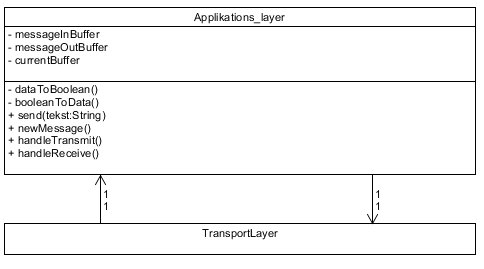
\includegraphics[scale=0.6]{Billeder/ApplicationLayerDesignClass.PNG}
\caption{Uddrag af designklassediagram med applikationslagets essentielle metoder og attributter}
\label{fig:AppLayerDesign}
\end{figure}
	

\subsection{Buffere}
Alle buffere på applikationslaget er deque-containere implementeret som first-in-first-out buffere - deques er mere effektive end vektorer, hvis data tages ud fra starten af bufferen. På afsendersiden bliver der brugt to buffere - den ene er en kø, hvor beskeder bliver gemt, når de bliver sendt fra brugeren med funktionen \textit{send()}. Den anden er bindeledet til transportlaget, og indeholder den næste besked der skal sendes. Inden beskeden kommer til denne bufferen, bliver den oversat til bools. Det er nødvendigt at have den i en buffer, hvis den er så stor at den skal skæres op i mindre stykker. Elementerne i bufferen er pointere til vektorerne. På modtagersiden bruges der kun en buffer, som brugeren kan polle for at hente beskeder ud. Beskeder der kommer op fra transportlaget som bools, bliver oversat til en streng som bliver flyttet til bufferen, når længden af den, matcher den der er givet i de 32 første bits.

\subsection{Afsender}
Metoden \textit{handleTransmit()} tager sig af at sende beskeder videre til transportlaget. Vektorer af bools bliver skubbet ned i transportlagets buffer, hvis den er tom. Når en hel besked er givet videre til transportlaget, bliver en ny hentet ned fra køen med metoden \textit{newMessage()}. Den sørger for at oversætte beskeden fra data til bools, placere længden af beskeden i de første 32 bits og at skære den i mindre stykker, hvis den er for stor.

\subsection{Modtager}
Metoden \textit{handleReceive()} sørger for at hente beskeder op fra en kø i transportlaget. En af de vigtige ting på modtagersiden, er at holde styr på hvornår en ny besked kommer ind, og hvornår den ender. Når den første besked kommer op fra transportlaget, findes længden for hele beskeden i de 32 første bits og gemmes som en lokal variabel i klassen. Hver gang der kommer noget nyt ind, kontrolleres længden, og når den overskrider det, skubbes beskeden til modtagerbufferen og den forventede længde nulstilles. 

\subsection{Generel drift}
Applikationslaget køres i sin egen tråd med metoden \textit{loop()}, der i en løkke sørger for skiftevis at køre \textit{handleReceive()} og \textit{handleTransmit()}. På den måde bliver alle buffere opdateret lige så snart  der sker noget nyt i transportlaget, eller brugeren sender en ny besked ind i systemet.